\documentclass{article} % For LaTeX2e
\usepackage{iclr2025,times}

% Optional math commands from https://github.com/goodfeli/dlbook_notation.
%%%%% NEW MATH DEFINITIONS %%%%%

\usepackage{amsmath,amsfonts,bm}

% Mark sections of captions for referring to divisions of figures
\newcommand{\figleft}{{\em (Left)}}
\newcommand{\figcenter}{{\em (Center)}}
\newcommand{\figright}{{\em (Right)}}
\newcommand{\figtop}{{\em (Top)}}
\newcommand{\figbottom}{{\em (Bottom)}}
\newcommand{\captiona}{{\em (a)}}
\newcommand{\captionb}{{\em (b)}}
\newcommand{\captionc}{{\em (c)}}
\newcommand{\captiond}{{\em (d)}}

% Highlight a newly defined term
\newcommand{\newterm}[1]{{\bf #1}}


% Figure reference, lower-case.
\def\figref#1{figure~\ref{#1}}
% Figure reference, capital. For start of sentence
\def\Figref#1{Figure~\ref{#1}}
\def\twofigref#1#2{figures \ref{#1} and \ref{#2}}
\def\quadfigref#1#2#3#4{figures \ref{#1}, \ref{#2}, \ref{#3} and \ref{#4}}
% Section reference, lower-case.
\def\secref#1{section~\ref{#1}}
% Section reference, capital.
\def\Secref#1{Section~\ref{#1}}
% Reference to two sections.
\def\twosecrefs#1#2{sections \ref{#1} and \ref{#2}}
% Reference to three sections.
\def\secrefs#1#2#3{sections \ref{#1}, \ref{#2} and \ref{#3}}
% Reference to an equation, lower-case.
\def\eqref#1{equation~\ref{#1}}
% Reference to an equation, upper case
\def\Eqref#1{Equation~\ref{#1}}
% A raw reference to an equation---avoid using if possible
\def\plaineqref#1{\ref{#1}}
% Reference to a chapter, lower-case.
\def\chapref#1{chapter~\ref{#1}}
% Reference to an equation, upper case.
\def\Chapref#1{Chapter~\ref{#1}}
% Reference to a range of chapters
\def\rangechapref#1#2{chapters\ref{#1}--\ref{#2}}
% Reference to an algorithm, lower-case.
\def\algref#1{algorithm~\ref{#1}}
% Reference to an algorithm, upper case.
\def\Algref#1{Algorithm~\ref{#1}}
\def\twoalgref#1#2{algorithms \ref{#1} and \ref{#2}}
\def\Twoalgref#1#2{Algorithms \ref{#1} and \ref{#2}}
% Reference to a part, lower case
\def\partref#1{part~\ref{#1}}
% Reference to a part, upper case
\def\Partref#1{Part~\ref{#1}}
\def\twopartref#1#2{parts \ref{#1} and \ref{#2}}

\def\ceil#1{\lceil #1 \rceil}
\def\floor#1{\lfloor #1 \rfloor}
\def\1{\bm{1}}
\newcommand{\train}{\mathcal{D}}
\newcommand{\valid}{\mathcal{D_{\mathrm{valid}}}}
\newcommand{\test}{\mathcal{D_{\mathrm{test}}}}

\def\eps{{\epsilon}}


% Random variables
\def\reta{{\textnormal{$\eta$}}}
\def\ra{{\textnormal{a}}}
\def\rb{{\textnormal{b}}}
\def\rc{{\textnormal{c}}}
\def\rd{{\textnormal{d}}}
\def\re{{\textnormal{e}}}
\def\rf{{\textnormal{f}}}
\def\rg{{\textnormal{g}}}
\def\rh{{\textnormal{h}}}
\def\ri{{\textnormal{i}}}
\def\rj{{\textnormal{j}}}
\def\rk{{\textnormal{k}}}
\def\rl{{\textnormal{l}}}
% rm is already a command, just don't name any random variables m
\def\rn{{\textnormal{n}}}
\def\ro{{\textnormal{o}}}
\def\rp{{\textnormal{p}}}
\def\rq{{\textnormal{q}}}
\def\rr{{\textnormal{r}}}
\def\rs{{\textnormal{s}}}
\def\rt{{\textnormal{t}}}
\def\ru{{\textnormal{u}}}
\def\rv{{\textnormal{v}}}
\def\rw{{\textnormal{w}}}
\def\rx{{\textnormal{x}}}
\def\ry{{\textnormal{y}}}
\def\rz{{\textnormal{z}}}

% Random vectors
\def\rvepsilon{{\mathbf{\epsilon}}}
\def\rvtheta{{\mathbf{\theta}}}
\def\rva{{\mathbf{a}}}
\def\rvb{{\mathbf{b}}}
\def\rvc{{\mathbf{c}}}
\def\rvd{{\mathbf{d}}}
\def\rve{{\mathbf{e}}}
\def\rvf{{\mathbf{f}}}
\def\rvg{{\mathbf{g}}}
\def\rvh{{\mathbf{h}}}
\def\rvu{{\mathbf{i}}}
\def\rvj{{\mathbf{j}}}
\def\rvk{{\mathbf{k}}}
\def\rvl{{\mathbf{l}}}
\def\rvm{{\mathbf{m}}}
\def\rvn{{\mathbf{n}}}
\def\rvo{{\mathbf{o}}}
\def\rvp{{\mathbf{p}}}
\def\rvq{{\mathbf{q}}}
\def\rvr{{\mathbf{r}}}
\def\rvs{{\mathbf{s}}}
\def\rvt{{\mathbf{t}}}
\def\rvu{{\mathbf{u}}}
\def\rvv{{\mathbf{v}}}
\def\rvw{{\mathbf{w}}}
\def\rvx{{\mathbf{x}}}
\def\rvy{{\mathbf{y}}}
\def\rvz{{\mathbf{z}}}

% Elements of random vectors
\def\erva{{\textnormal{a}}}
\def\ervb{{\textnormal{b}}}
\def\ervc{{\textnormal{c}}}
\def\ervd{{\textnormal{d}}}
\def\erve{{\textnormal{e}}}
\def\ervf{{\textnormal{f}}}
\def\ervg{{\textnormal{g}}}
\def\ervh{{\textnormal{h}}}
\def\ervi{{\textnormal{i}}}
\def\ervj{{\textnormal{j}}}
\def\ervk{{\textnormal{k}}}
\def\ervl{{\textnormal{l}}}
\def\ervm{{\textnormal{m}}}
\def\ervn{{\textnormal{n}}}
\def\ervo{{\textnormal{o}}}
\def\ervp{{\textnormal{p}}}
\def\ervq{{\textnormal{q}}}
\def\ervr{{\textnormal{r}}}
\def\ervs{{\textnormal{s}}}
\def\ervt{{\textnormal{t}}}
\def\ervu{{\textnormal{u}}}
\def\ervv{{\textnormal{v}}}
\def\ervw{{\textnormal{w}}}
\def\ervx{{\textnormal{x}}}
\def\ervy{{\textnormal{y}}}
\def\ervz{{\textnormal{z}}}

% Random matrices
\def\rmA{{\mathbf{A}}}
\def\rmB{{\mathbf{B}}}
\def\rmC{{\mathbf{C}}}
\def\rmD{{\mathbf{D}}}
\def\rmE{{\mathbf{E}}}
\def\rmF{{\mathbf{F}}}
\def\rmG{{\mathbf{G}}}
\def\rmH{{\mathbf{H}}}
\def\rmI{{\mathbf{I}}}
\def\rmJ{{\mathbf{J}}}
\def\rmK{{\mathbf{K}}}
\def\rmL{{\mathbf{L}}}
\def\rmM{{\mathbf{M}}}
\def\rmN{{\mathbf{N}}}
\def\rmO{{\mathbf{O}}}
\def\rmP{{\mathbf{P}}}
\def\rmQ{{\mathbf{Q}}}
\def\rmR{{\mathbf{R}}}
\def\rmS{{\mathbf{S}}}
\def\rmT{{\mathbf{T}}}
\def\rmU{{\mathbf{U}}}
\def\rmV{{\mathbf{V}}}
\def\rmW{{\mathbf{W}}}
\def\rmX{{\mathbf{X}}}
\def\rmY{{\mathbf{Y}}}
\def\rmZ{{\mathbf{Z}}}

% Elements of random matrices
\def\ermA{{\textnormal{A}}}
\def\ermB{{\textnormal{B}}}
\def\ermC{{\textnormal{C}}}
\def\ermD{{\textnormal{D}}}
\def\ermE{{\textnormal{E}}}
\def\ermF{{\textnormal{F}}}
\def\ermG{{\textnormal{G}}}
\def\ermH{{\textnormal{H}}}
\def\ermI{{\textnormal{I}}}
\def\ermJ{{\textnormal{J}}}
\def\ermK{{\textnormal{K}}}
\def\ermL{{\textnormal{L}}}
\def\ermM{{\textnormal{M}}}
\def\ermN{{\textnormal{N}}}
\def\ermO{{\textnormal{O}}}
\def\ermP{{\textnormal{P}}}
\def\ermQ{{\textnormal{Q}}}
\def\ermR{{\textnormal{R}}}
\def\ermS{{\textnormal{S}}}
\def\ermT{{\textnormal{T}}}
\def\ermU{{\textnormal{U}}}
\def\ermV{{\textnormal{V}}}
\def\ermW{{\textnormal{W}}}
\def\ermX{{\textnormal{X}}}
\def\ermY{{\textnormal{Y}}}
\def\ermZ{{\textnormal{Z}}}

% Vectors
\def\vzero{{\bm{0}}}
\def\vone{{\bm{1}}}
\def\vmu{{\bm{\mu}}}
\def\vtheta{{\bm{\theta}}}
\def\va{{\bm{a}}}
\def\vb{{\bm{b}}}
\def\vc{{\bm{c}}}
\def\vd{{\bm{d}}}
\def\ve{{\bm{e}}}
\def\vf{{\bm{f}}}
\def\vg{{\bm{g}}}
\def\vh{{\bm{h}}}
\def\vi{{\bm{i}}}
\def\vj{{\bm{j}}}
\def\vk{{\bm{k}}}
\def\vl{{\bm{l}}}
\def\vm{{\bm{m}}}
\def\vn{{\bm{n}}}
\def\vo{{\bm{o}}}
\def\vp{{\bm{p}}}
\def\vq{{\bm{q}}}
\def\vr{{\bm{r}}}
\def\vs{{\bm{s}}}
\def\vt{{\bm{t}}}
\def\vu{{\bm{u}}}
\def\vv{{\bm{v}}}
\def\vw{{\bm{w}}}
\def\vx{{\bm{x}}}
\def\vy{{\bm{y}}}
\def\vz{{\bm{z}}}

% Elements of vectors
\def\evalpha{{\alpha}}
\def\evbeta{{\beta}}
\def\evepsilon{{\epsilon}}
\def\evlambda{{\lambda}}
\def\evomega{{\omega}}
\def\evmu{{\mu}}
\def\evpsi{{\psi}}
\def\evsigma{{\sigma}}
\def\evtheta{{\theta}}
\def\eva{{a}}
\def\evb{{b}}
\def\evc{{c}}
\def\evd{{d}}
\def\eve{{e}}
\def\evf{{f}}
\def\evg{{g}}
\def\evh{{h}}
\def\evi{{i}}
\def\evj{{j}}
\def\evk{{k}}
\def\evl{{l}}
\def\evm{{m}}
\def\evn{{n}}
\def\evo{{o}}
\def\evp{{p}}
\def\evq{{q}}
\def\evr{{r}}
\def\evs{{s}}
\def\evt{{t}}
\def\evu{{u}}
\def\evv{{v}}
\def\evw{{w}}
\def\evx{{x}}
\def\evy{{y}}
\def\evz{{z}}

% Matrix
\def\mA{{\bm{A}}}
\def\mB{{\bm{B}}}
\def\mC{{\bm{C}}}
\def\mD{{\bm{D}}}
\def\mE{{\bm{E}}}
\def\mF{{\bm{F}}}
\def\mG{{\bm{G}}}
\def\mH{{\bm{H}}}
\def\mI{{\bm{I}}}
\def\mJ{{\bm{J}}}
\def\mK{{\bm{K}}}
\def\mL{{\bm{L}}}
\def\mM{{\bm{M}}}
\def\mN{{\bm{N}}}
\def\mO{{\bm{O}}}
\def\mP{{\bm{P}}}
\def\mQ{{\bm{Q}}}
\def\mR{{\bm{R}}}
\def\mS{{\bm{S}}}
\def\mT{{\bm{T}}}
\def\mU{{\bm{U}}}
\def\mV{{\bm{V}}}
\def\mW{{\bm{W}}}
\def\mX{{\bm{X}}}
\def\mY{{\bm{Y}}}
\def\mZ{{\bm{Z}}}
\def\mBeta{{\bm{\beta}}}
\def\mPhi{{\bm{\Phi}}}
\def\mLambda{{\bm{\Lambda}}}
\def\mSigma{{\bm{\Sigma}}}

% Tensor
\DeclareMathAlphabet{\mathsfit}{\encodingdefault}{\sfdefault}{m}{sl}
\SetMathAlphabet{\mathsfit}{bold}{\encodingdefault}{\sfdefault}{bx}{n}
\newcommand{\tens}[1]{\bm{\mathsfit{#1}}}
\def\tA{{\tens{A}}}
\def\tB{{\tens{B}}}
\def\tC{{\tens{C}}}
\def\tD{{\tens{D}}}
\def\tE{{\tens{E}}}
\def\tF{{\tens{F}}}
\def\tG{{\tens{G}}}
\def\tH{{\tens{H}}}
\def\tI{{\tens{I}}}
\def\tJ{{\tens{J}}}
\def\tK{{\tens{K}}}
\def\tL{{\tens{L}}}
\def\tM{{\tens{M}}}
\def\tN{{\tens{N}}}
\def\tO{{\tens{O}}}
\def\tP{{\tens{P}}}
\def\tQ{{\tens{Q}}}
\def\tR{{\tens{R}}}
\def\tS{{\tens{S}}}
\def\tT{{\tens{T}}}
\def\tU{{\tens{U}}}
\def\tV{{\tens{V}}}
\def\tW{{\tens{W}}}
\def\tX{{\tens{X}}}
\def\tY{{\tens{Y}}}
\def\tZ{{\tens{Z}}}


% Graph
\def\gA{{\mathcal{A}}}
\def\gB{{\mathcal{B}}}
\def\gC{{\mathcal{C}}}
\def\gD{{\mathcal{D}}}
\def\gE{{\mathcal{E}}}
\def\gF{{\mathcal{F}}}
\def\gG{{\mathcal{G}}}
\def\gH{{\mathcal{H}}}
\def\gI{{\mathcal{I}}}
\def\gJ{{\mathcal{J}}}
\def\gK{{\mathcal{K}}}
\def\gL{{\mathcal{L}}}
\def\gM{{\mathcal{M}}}
\def\gN{{\mathcal{N}}}
\def\gO{{\mathcal{O}}}
\def\gP{{\mathcal{P}}}
\def\gQ{{\mathcal{Q}}}
\def\gR{{\mathcal{R}}}
\def\gS{{\mathcal{S}}}
\def\gT{{\mathcal{T}}}
\def\gU{{\mathcal{U}}}
\def\gV{{\mathcal{V}}}
\def\gW{{\mathcal{W}}}
\def\gX{{\mathcal{X}}}
\def\gY{{\mathcal{Y}}}
\def\gZ{{\mathcal{Z}}}

% Sets
\def\sA{{\mathbb{A}}}
\def\sB{{\mathbb{B}}}
\def\sC{{\mathbb{C}}}
\def\sD{{\mathbb{D}}}
% Don't use a set called E, because this would be the same as our symbol
% for expectation.
\def\sF{{\mathbb{F}}}
\def\sG{{\mathbb{G}}}
\def\sH{{\mathbb{H}}}
\def\sI{{\mathbb{I}}}
\def\sJ{{\mathbb{J}}}
\def\sK{{\mathbb{K}}}
\def\sL{{\mathbb{L}}}
\def\sM{{\mathbb{M}}}
\def\sN{{\mathbb{N}}}
\def\sO{{\mathbb{O}}}
\def\sP{{\mathbb{P}}}
\def\sQ{{\mathbb{Q}}}
\def\sR{{\mathbb{R}}}
\def\sS{{\mathbb{S}}}
\def\sT{{\mathbb{T}}}
\def\sU{{\mathbb{U}}}
\def\sV{{\mathbb{V}}}
\def\sW{{\mathbb{W}}}
\def\sX{{\mathbb{X}}}
\def\sY{{\mathbb{Y}}}
\def\sZ{{\mathbb{Z}}}

% Entries of a matrix
\def\emLambda{{\Lambda}}
\def\emA{{A}}
\def\emB{{B}}
\def\emC{{C}}
\def\emD{{D}}
\def\emE{{E}}
\def\emF{{F}}
\def\emG{{G}}
\def\emH{{H}}
\def\emI{{I}}
\def\emJ{{J}}
\def\emK{{K}}
\def\emL{{L}}
\def\emM{{M}}
\def\emN{{N}}
\def\emO{{O}}
\def\emP{{P}}
\def\emQ{{Q}}
\def\emR{{R}}
\def\emS{{S}}
\def\emT{{T}}
\def\emU{{U}}
\def\emV{{V}}
\def\emW{{W}}
\def\emX{{X}}
\def\emY{{Y}}
\def\emZ{{Z}}
\def\emSigma{{\Sigma}}

% entries of a tensor
% Same font as tensor, without \bm wrapper
\newcommand{\etens}[1]{\mathsfit{#1}}
\def\etLambda{{\etens{\Lambda}}}
\def\etA{{\etens{A}}}
\def\etB{{\etens{B}}}
\def\etC{{\etens{C}}}
\def\etD{{\etens{D}}}
\def\etE{{\etens{E}}}
\def\etF{{\etens{F}}}
\def\etG{{\etens{G}}}
\def\etH{{\etens{H}}}
\def\etI{{\etens{I}}}
\def\etJ{{\etens{J}}}
\def\etK{{\etens{K}}}
\def\etL{{\etens{L}}}
\def\etM{{\etens{M}}}
\def\etN{{\etens{N}}}
\def\etO{{\etens{O}}}
\def\etP{{\etens{P}}}
\def\etQ{{\etens{Q}}}
\def\etR{{\etens{R}}}
\def\etS{{\etens{S}}}
\def\etT{{\etens{T}}}
\def\etU{{\etens{U}}}
\def\etV{{\etens{V}}}
\def\etW{{\etens{W}}}
\def\etX{{\etens{X}}}
\def\etY{{\etens{Y}}}
\def\etZ{{\etens{Z}}}

% The true underlying data generating distribution
\newcommand{\pdata}{p_{\rm{data}}}
% The empirical distribution defined by the training set
\newcommand{\ptrain}{\hat{p}_{\rm{data}}}
\newcommand{\Ptrain}{\hat{P}_{\rm{data}}}
% The model distribution
\newcommand{\pmodel}{p_{\rm{model}}}
\newcommand{\Pmodel}{P_{\rm{model}}}
\newcommand{\ptildemodel}{\tilde{p}_{\rm{model}}}
% Stochastic autoencoder distributions
\newcommand{\pencode}{p_{\rm{encoder}}}
\newcommand{\pdecode}{p_{\rm{decoder}}}
\newcommand{\precons}{p_{\rm{reconstruct}}}

\newcommand{\laplace}{\mathrm{Laplace}} % Laplace distribution

\newcommand{\E}{\mathbb{E}}
\newcommand{\Ls}{\mathcal{L}}
\newcommand{\R}{\mathbb{R}}
\newcommand{\emp}{\tilde{p}}
\newcommand{\lr}{\alpha}
\newcommand{\reg}{\lambda}
\newcommand{\rect}{\mathrm{rectifier}}
\newcommand{\softmax}{\mathrm{softmax}}
\newcommand{\sigmoid}{\sigma}
\newcommand{\softplus}{\zeta}
\newcommand{\KL}{D_{\mathrm{KL}}}
\newcommand{\Var}{\mathrm{Var}}
\newcommand{\standarderror}{\mathrm{SE}}
\newcommand{\Cov}{\mathrm{Cov}}
% Wolfram Mathworld says $L^2$ is for function spaces and $\ell^2$ is for vectors
% But then they seem to use $L^2$ for vectors throughout the site, and so does
% wikipedia.
\newcommand{\normlzero}{L^0}
\newcommand{\normlone}{L^1}
\newcommand{\normltwo}{L^2}
\newcommand{\normlp}{L^p}
\newcommand{\normmax}{L^\infty}

\newcommand{\parents}{Pa} % See usage in notation.tex. Chosen to match Daphne's book.

\DeclareMathOperator*{\argmax}{arg\,max}
\DeclareMathOperator*{\argmin}{arg\,min}

\DeclareMathOperator{\sign}{sign}
\DeclareMathOperator{\Tr}{Tr}
\let\ab\allowbreak


\usepackage{hyperref}
\usepackage{url}
\usepackage{graphicx}
\usepackage{subfigure}
\usepackage{booktabs}

% For theorems and such
\usepackage{amsmath}
\usepackage{amssymb}
\usepackage{mathtools}
\usepackage{amsthm}

% Custom
\usepackage{multirow}
\usepackage{color}
\usepackage{colortbl}
\usepackage[capitalize,noabbrev]{cleveref}
\usepackage{xspace}

%%%%%%%%%%%%%%%%%%%%%%%%%%%%%%%%
% THEOREMS
%%%%%%%%%%%%%%%%%%%%%%%%%%%%%%%%
\theoremstyle{plain}
\newtheorem{theorem}{Theorem}[section]
\newtheorem{proposition}[theorem]{Proposition}
\newtheorem{lemma}[theorem]{Lemma}
\newtheorem{corollary}[theorem]{Corollary}
\theoremstyle{definition}
\newtheorem{definition}[theorem]{Definition}
\newtheorem{assumption}[theorem]{Assumption}
\theoremstyle{remark}
\newtheorem{remark}[theorem]{Remark}

\graphicspath{{../figures/}} % DO NOT CHANGE THIS.

\begin{filecontents}{references.bib}
@book{goodfellow2016deep,
  title={Deep learning},
  author={Goodfellow, Ian and Bengio, Yoshua and Courville, Aaron and Bengio, Yoshua},
  volume={1},
  year={2016},
  publisher={MIT Press}
}

@inproceedings{hamerly2017acceleratingla,
 author = {Greg Hamerly and Jonathan Drake},
 title = {Accelerating Lloyd's Algorithm for k-Means Clustering},
 year = {2017}
}

@article{devlin2019bertpo,
 author = {Jacob Devlin and Ming-Wei Chang and Kenton Lee and Kristina Toutanova},
 booktitle = {North American Chapter of the Association for Computational Linguistics},
 pages = {4171-4186},
 title = {BERT: Pre-training of Deep Bidirectional Transformers for Language Understanding},
 year = {2019}
}

@article{shahapure2020clusterqa,
 author = {K. Shahapure and Charles K. Nicholas},
 booktitle = {International Conference on Data Science and Advanced Analytics},
 journal = {2020 IEEE 7th International Conference on Data Science and Advanced Analytics (DSAA)},
 pages = {747-748},
 title = {Cluster Quality Analysis Using Silhouette Score},
 year = {2020}
}

@article{weis2020benchmarkinguo,
 author = {Marissa A. Weis and Kashyap Chitta and Yash Sharma and Wieland Brendel and M. Bethge and Andreas Geiger and Alexander S. Ecker},
 booktitle = {Journal of machine learning research},
 journal = {J. Mach. Learn. Res.},
 pages = {183:1-183:61},
 title = {Benchmarking Unsupervised Object Representations for Video Sequences},
 volume = {22},
 year = {2020}
}

@article{rajotia2025principalca,
 author = {Meghana Singh Rajotia and D. Vart and A. Dashora and Rao Pankaj and Harshdeep and Jyoti , Neeraj Kharor and S. K. Pahuja},
 booktitle = {Ecology, environment & conservation},
 journal = {Ecology, Environment and Conservation},
 title = {Principal Component Analysis approach for Rancidity and Grain Yield Traits in Pearl Millet},
 year = {2025}
}

@article{snell2017prototypicalnf,
 author = {Jake Snell and Kevin Swersky and R. Zemel},
 booktitle = {Neural Information Processing Systems},
 pages = {4077-4087},
 title = {Prototypical Networks for Few-shot Learning},
 year = {2017}
}

@article{barbiero2023interpretablenc,
 author = {Pietro Barbiero and Gabriele Ciravegna and Francesco Giannini and Mateo Espinosa Zarlenga and Lucie Charlotte Magister and A. Tonda and Pietro Lio' and F. Precioso and M. Jamnik and G. Marra},
 booktitle = {International Workshop on Neural-Symbolic Learning and Reasoning},
 journal = {ArXiv},
 title = {Interpretable Neural-Symbolic Concept Reasoning},
 volume = {abs/2304.14068},
 year = {2023}
}

@article{jeong2025symbolnetbl,
 author = {SungHeon Jeong and Hyungjoon Kim and Yoojeong Song},
 booktitle = {IEEE Access},
 journal = {IEEE Access},
 pages = {78221-78230},
 title = {SymbolNet: Bridging Latent Neural Representations and Symbolic Reasoning via Intermediate Feature Interpretation},
 volume = {13},
 year = {2025}
}

@article{morishita2024enhancingrc,
 author = {Terufumi Morishita and Gaku Morio and Atsuki Yamaguchi and Yasuhiro Sogawa},
 booktitle = {Neural Information Processing Systems},
 journal = {ArXiv},
 title = {Enhancing Reasoning Capabilities of LLMs via Principled Synthetic Logic Corpus},
 volume = {abs/2411.12498},
 year = {2024}
}

@article{bereta2025theso,
 author = {Pola Bereta and Ioannis Diamantis},
 booktitle = {arXiv.org},
 journal = {ArXiv},
 title = {The Shape of Consumer Behavior: A Symbolic and Topological Analysis of Time Series},
 volume = {abs/2506.19759},
 year = {2025}
}
\end{filecontents}

\title{Unveiling Hidden Patterns: Symbolic Glyph Clustering for Enhanced PolyRule Reasoning}

\author{Anonymous}

\begin{document}

\maketitle

\begin{abstract}
Symbolic Pattern Recognition (SPR) often involves deciphering latent rules from sequences of abstract glyphs. We investigate whether clustering glyphs based on latent feature representations can reveal hidden structure and improve reasoning performance. We propose a pipeline that uses pre-trained embeddings, clusters glyphs using K-means, then feeds the clustered representations into a neural reasoning model. Experiments on a synthetic SPR benchmark show partial improvements, particularly for shape-focused metrics, yet fail to surpass the state of the art on color-based tasks. The findings highlight the challenges and potential pitfalls in applying clustering to symbolic reasoning.
\end{abstract}

\section{Introduction}
\label{sec:intro}
Many real-world tasks involve abstract, symbolic manipulations, but neural models often struggle when symbols do not follow conventional text distributions. Synthetic datasets such as SPR\_BENCH facilitate controlled evaluation \citep{morishita2024enhancingrc}. Our focus is symbol clustering for improved reasoning. We hypothesize that grouping glyphs by shared features can reveal interpretable patterns. This can have implications for neural-symbolic integration \citep{barbiero2023interpretablenc, jeong2025symbolnetbl} and for bridging latent representations with more explicit structure \citep{goodfellow2016deep}.

We present a clustering-based approach for PolyRule reasoning: (1) latent feature extraction, (2) glyph grouping, and (3) aggregated reasoning. Despite strong performance on shape-dependent metrics, our approach underperforms on color-weighted tasks. These mixed results underscore the challenges of balancing multiple symbolic attributes.

\section{Related Work}
\label{sec:related}
Symbolic clustering has been explored in few-shot learning \citep{snell2017prototypicalnf} and unsupervised object representation tasks \citep{weis2020benchmarkinguo}, though prior studies primarily evaluated natural images or text rather than abstract glyphs. Dimensionality reduction (e.g., PCA) is often applied to mitigate computational costs when clustering large feature sets \citep{rajotia2025principalca}. We rely on K-means \citep{hamerly2017acceleratingla} and validate cluster quality using silhouette scores \citep{shahapure2020clusterqa}. Our work expands on neural-symbolic methodologies \citep{barbiero2023interpretablenc, jeong2025symbolnetbl} by focusing on a novel symbolic domain with color and shape attributes. Clustering high-entropy symbols can be ambiguous \citep{bereta2025theso}, leading to pitfalls in practice.

\section{Method}
\label{sec:method}
We load sequences from SPR\_BENCH, each symbol composed of shape and color tags, then tokenize them with a pre-trained model (e.g., BERT) \citep{devlin2019bertpo} or simple ID lookups. We optionally reduce dimensionality \citep{rajotia2025principalca} before clustering. K-means assigns each symbol to a cluster, producing a label used alongside the raw shape and color embeddings. A neural reasoning module (e.g., a BiLSTM) sums or concatenates embeddings, averages token representations, and classifies the rule. We train with cross-entropy on the labeled sequence, selecting the best checkpoint by validation loss.

\section{Experiments}
\label{sec:experiments}
We first compare a baseline model with embedding dimensions of 4--64. Validation scores increase slightly for higher dimensions, but final test metrics remain around 0.63--0.68 for color and shape. We then incorporate clustering. Shape-weighted accuracy (SWA) improves from 0.65 to 0.70, but color-weighted accuracy (CWA) remains at 0.635, short of the 0.70 state of the art. These differences suggest that simplistic clustering pipelines can more effectively capture shape cues than subtle color variations.

\begin{figure}[t!]
\centering
\subfigure[Baseline Dimension Tuning]{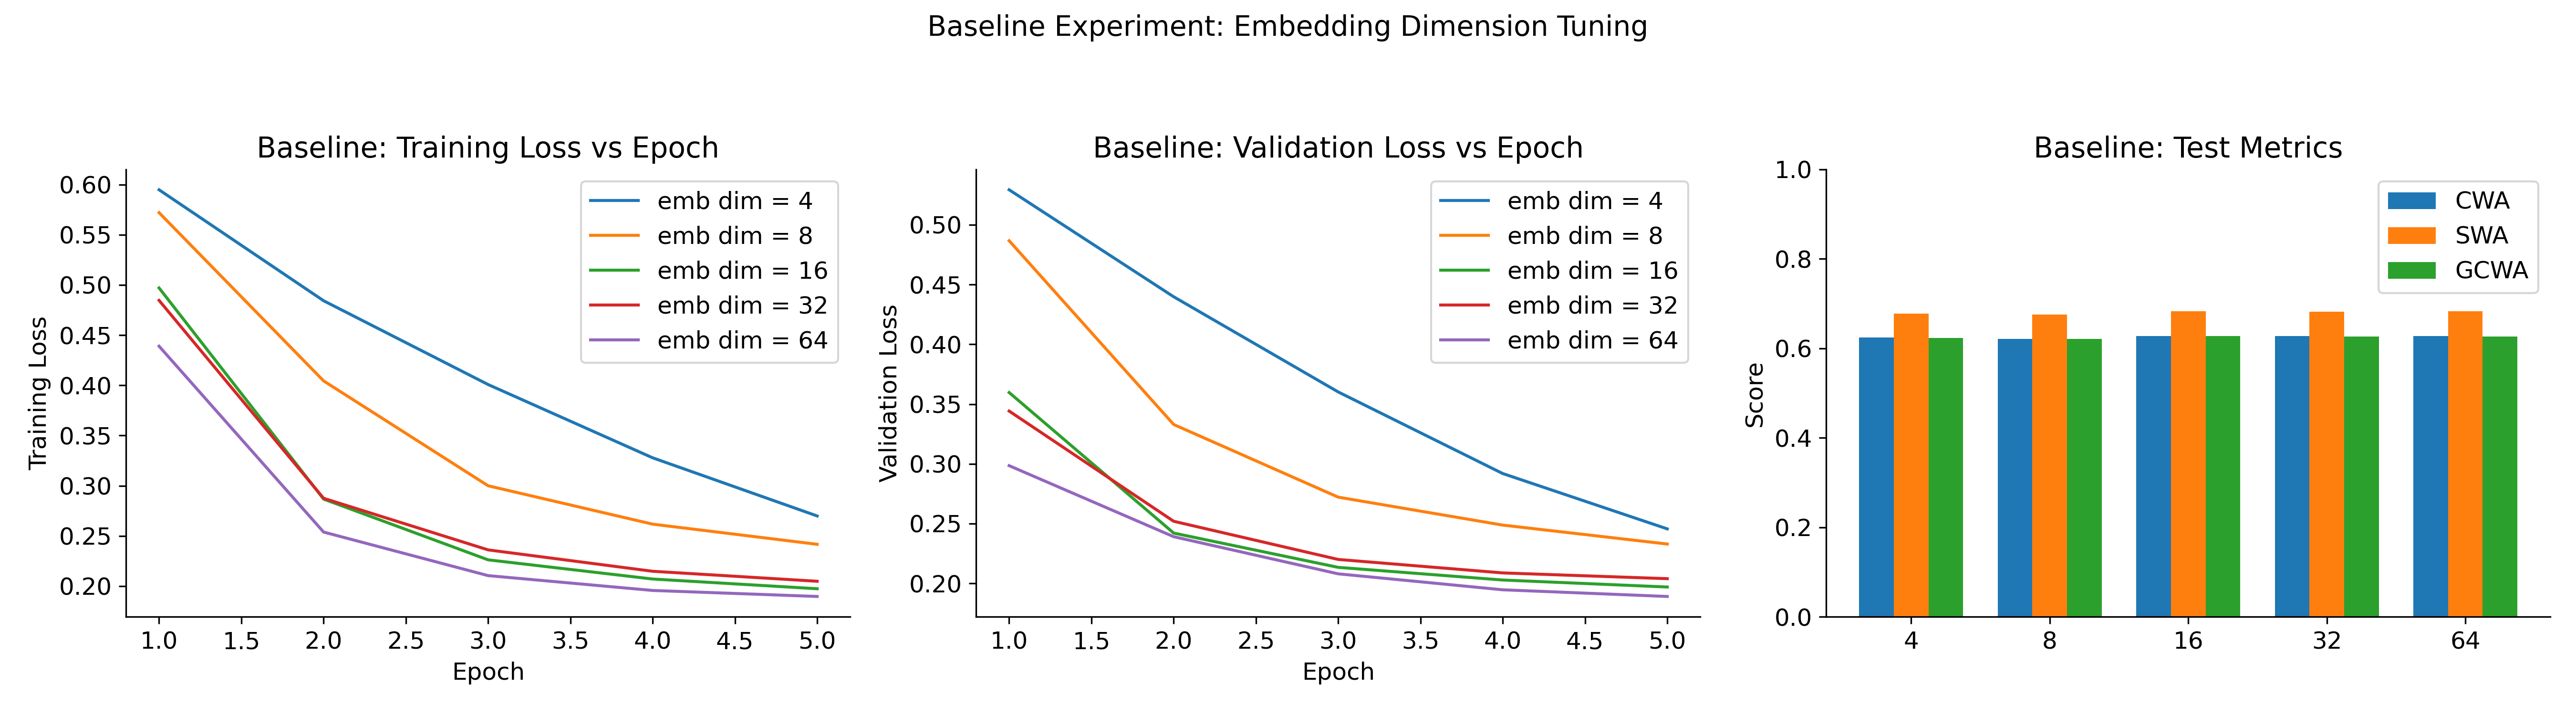
\includegraphics[width=0.33\textwidth]{baseline_embedding_dimension.png}\label{fig:baseline}}
\hfill
\subfigure[Enhanced BiLSTM + Clustering]{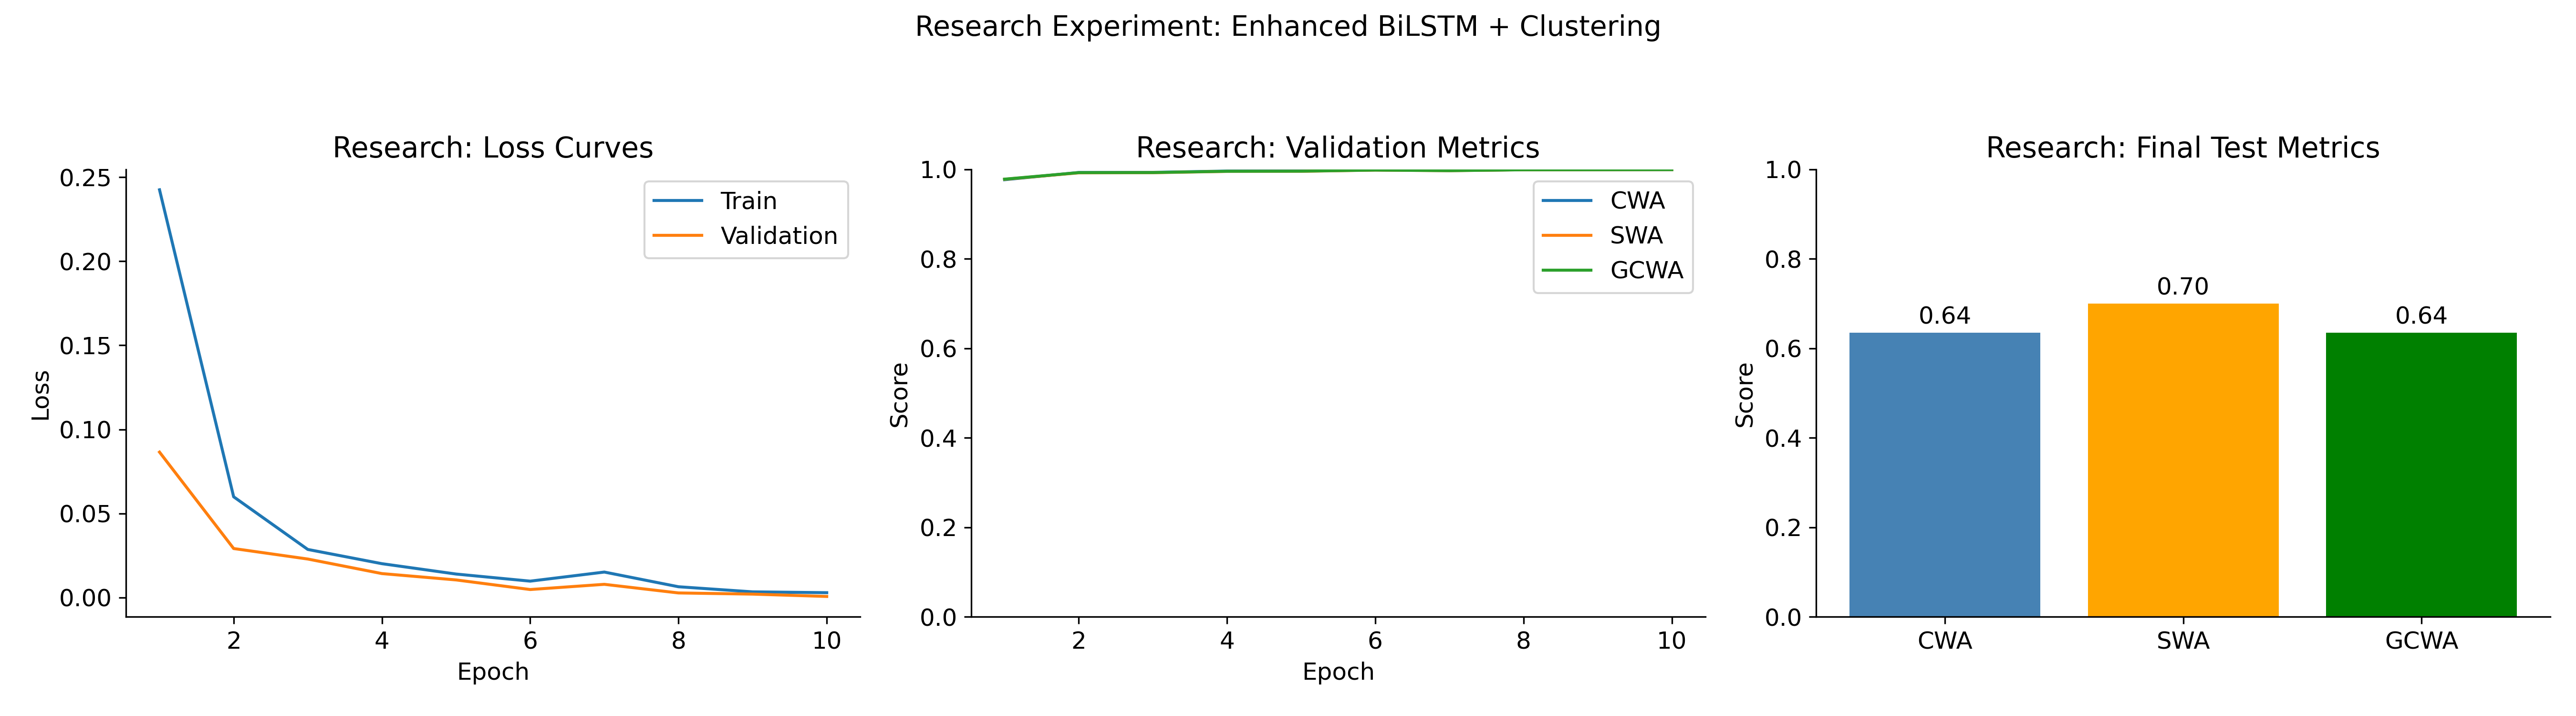
\includegraphics[width=0.33\textwidth]{research_enhanced_model.png}\label{fig:research}}
\caption{\textbf{Figure 1: Key experiment results on SPR\_BENCH.} (a) Minor gains from higher embedding dimensions. (b) BiLSTM plus glyph clustering improves shape-based metrics but struggles with color attributes. Overall, the right subfigure highlights how clustering is beneficial for certain attributes (e.g., shape) yet fails to strengthen color reasoning, indicating difficulties in multi-attribute symbolic tasks.}
\end{figure}

We used the Adam optimizer (learning rate 2e-4), batch size 32, and early stopping with patience of 5. In practice, we found that random initialization of cluster centroids sometimes produced local minima, suggesting that more careful cluster initialization or specialized distances may be required to fully capture color nuances.

\section{Conclusion}
\label{sec:conclusion}
Symbolic glyph clustering for reasoning reveals latent shape structure but fares worse on color attributes. This partially successful result underscores the complexity of symbolic tasks that incorporate multiple attributes. Future work might explore alternative distance metrics or specialized clustering. These findings encourage the community to share both promising and inconclusive directions, echoing the workshop's emphasis on real-world challenges and negative results in deep learning.

\bibliography{iclr2025}
\bibliographystyle{iclr2025}

\appendix

\section*{\LARGE Supplementary Material}
\label{sec:appendix}
Here, we provide ablation studies that demonstrate the effects of various design decisions, such as removing color embeddings, introducing random clusters, and altering the embedding fusion method. We show that each factor can meaningfully affect performance. Specifically, removing color embeddings or relying on random clustering degrades results, particularly on color-based tasks, while alternative embedding fusion (summation vs.\ concatenation) introduces trade-offs between shape focus and color fidelity. These comprehensive ablations underscore how subtle implementation details matter for symbolic pattern recognition pipelines.

\begin{figure}[h]
\centering
\subfigure[Atomic glyph embeddings]{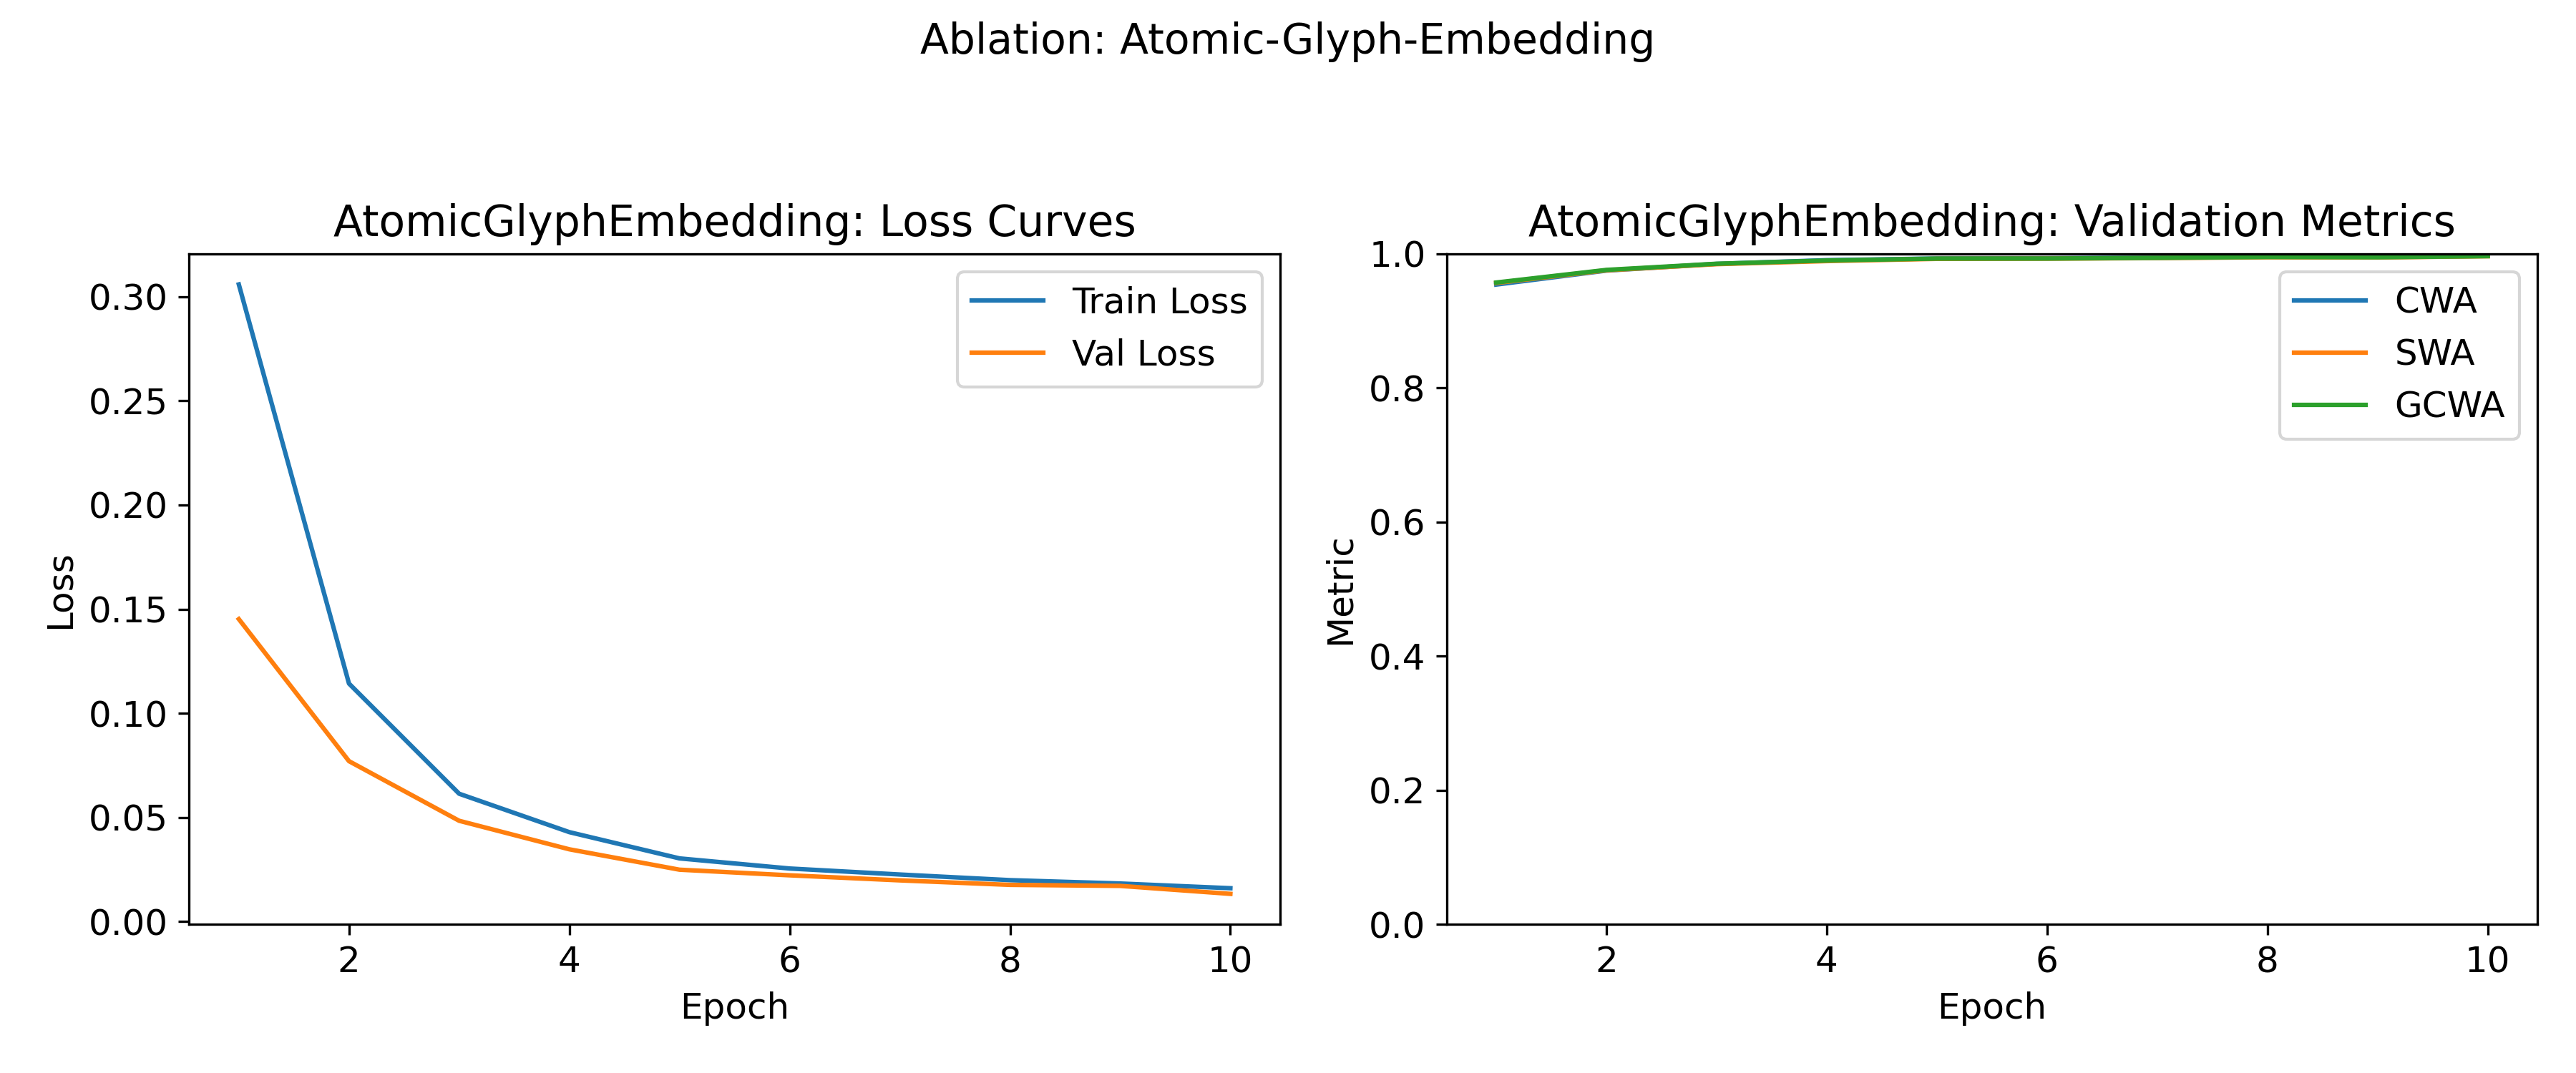
\includegraphics[width=0.24\textwidth]{ablation_atomic_glyph_embedding.png}\label{fig:ablations1}}
\subfigure[Bag-of-glyph approach]{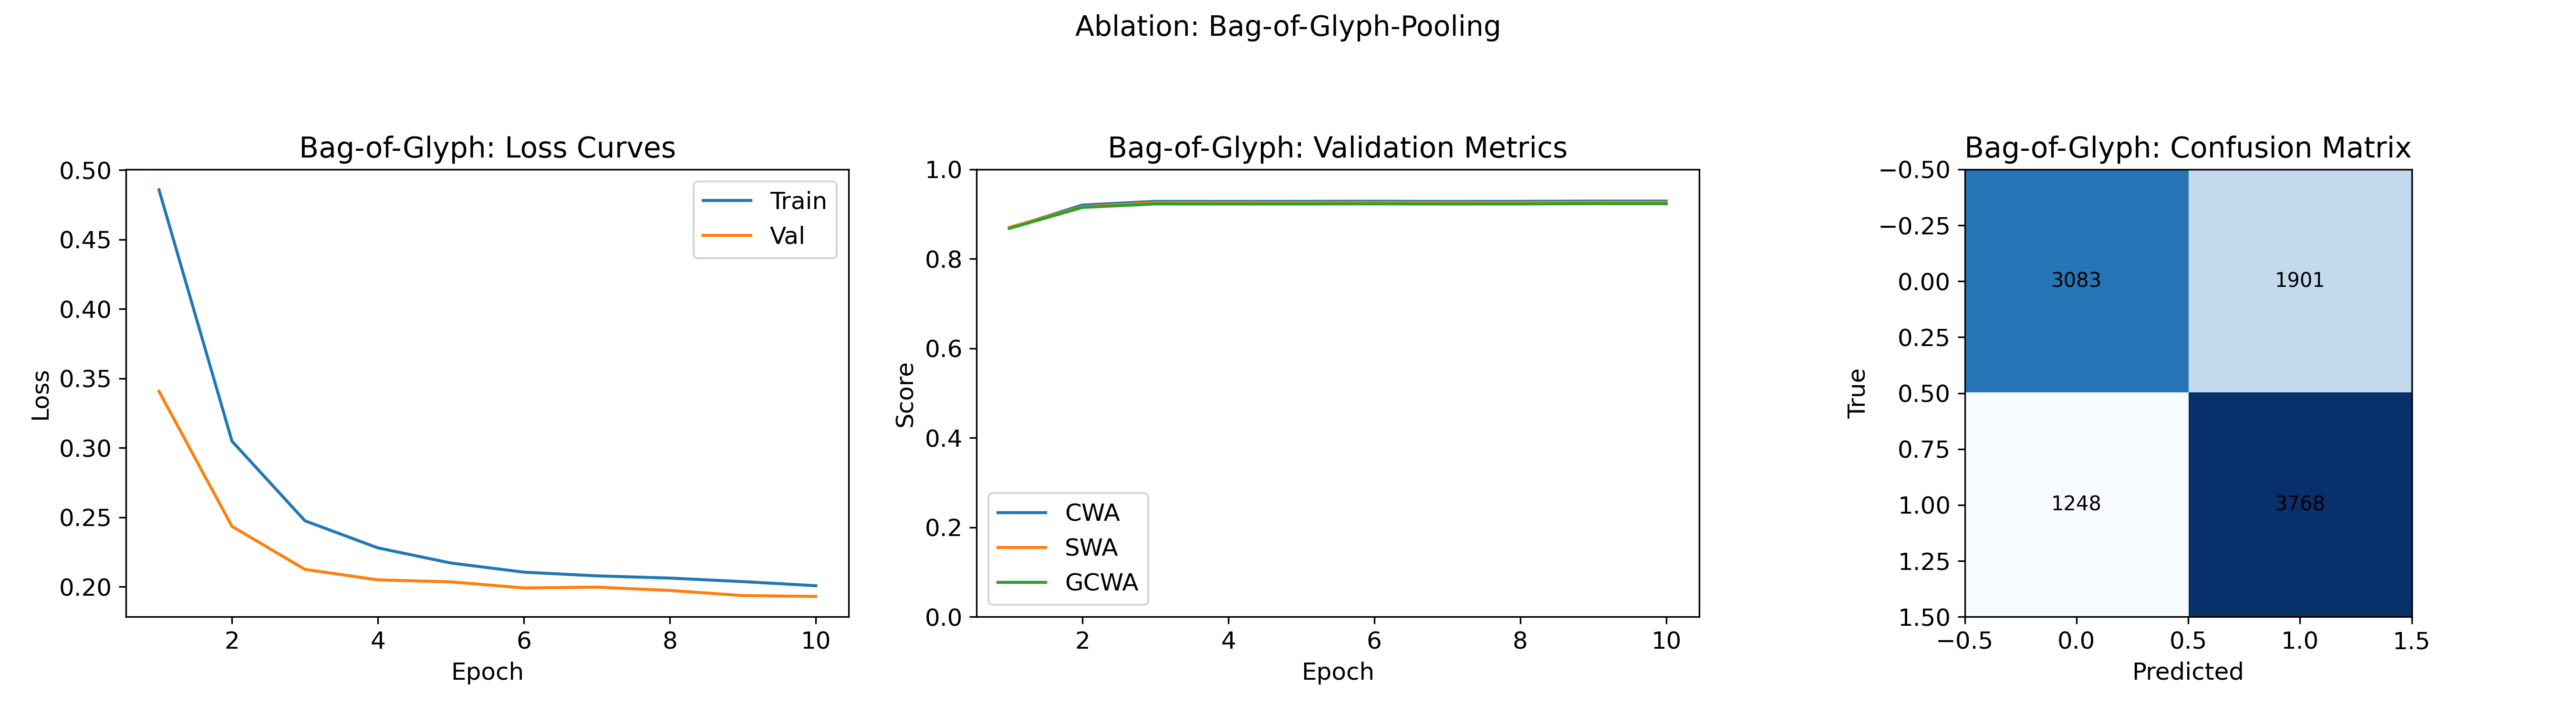
\includegraphics[width=0.24\textwidth]{ablation_bag_of_glyph.png}\label{fig:ablations2}}
\subfigure[Multi-synth training]{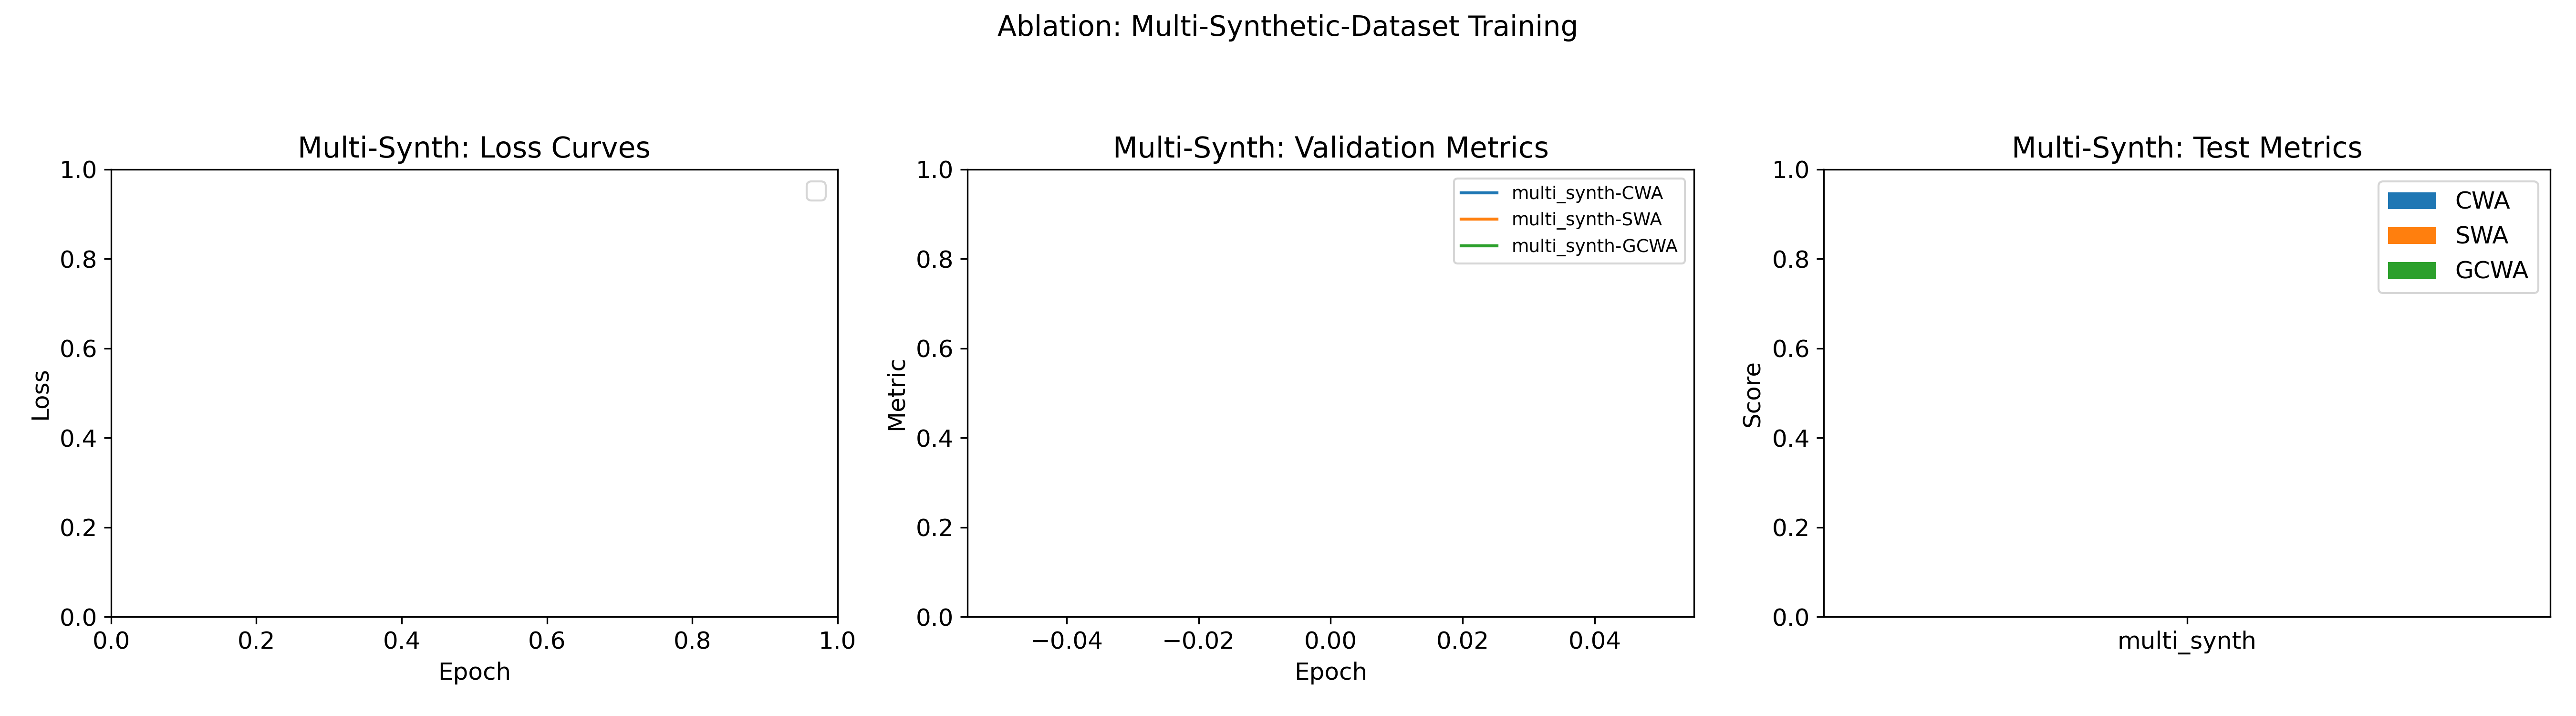
\includegraphics[width=0.24\textwidth]{ablation_multi_synth_training.png}\label{fig:ablations3}}
\subfigure[No cluster embedding]{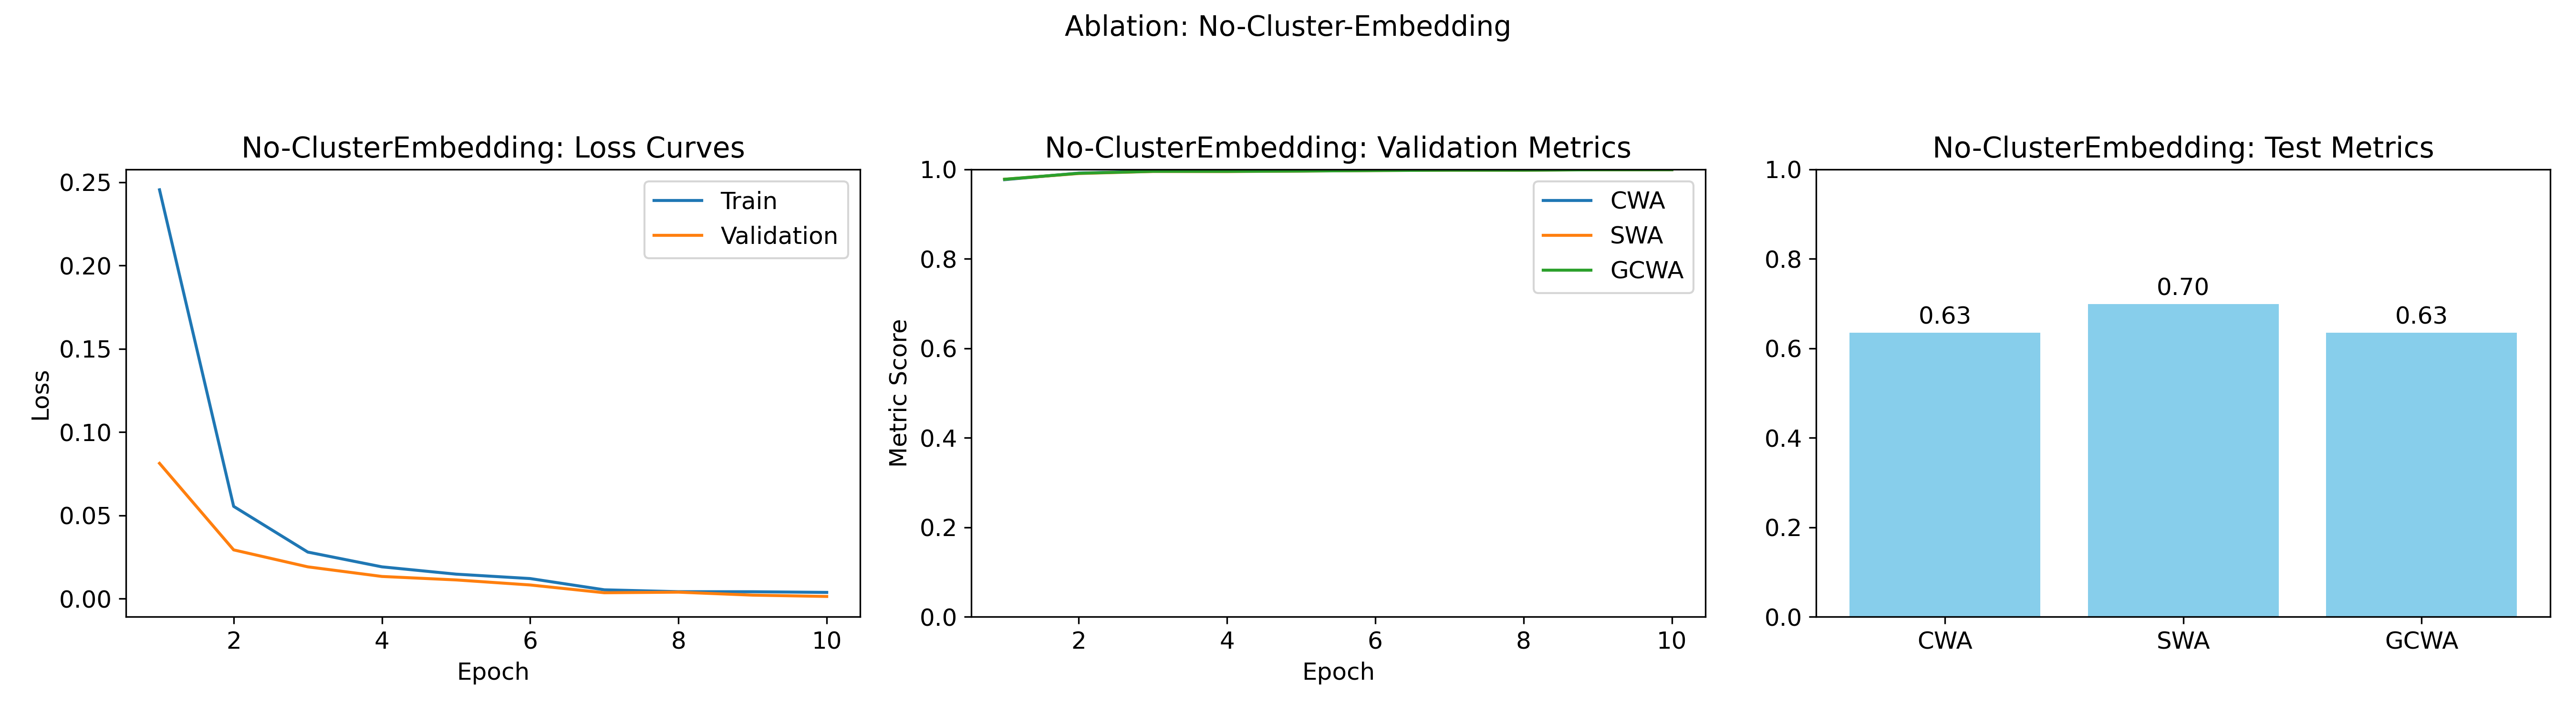
\includegraphics[width=0.24\textwidth]{ablation_no_cluster_embedding.png}\label{fig:ablations4}}
\subfigure[No color embedding]{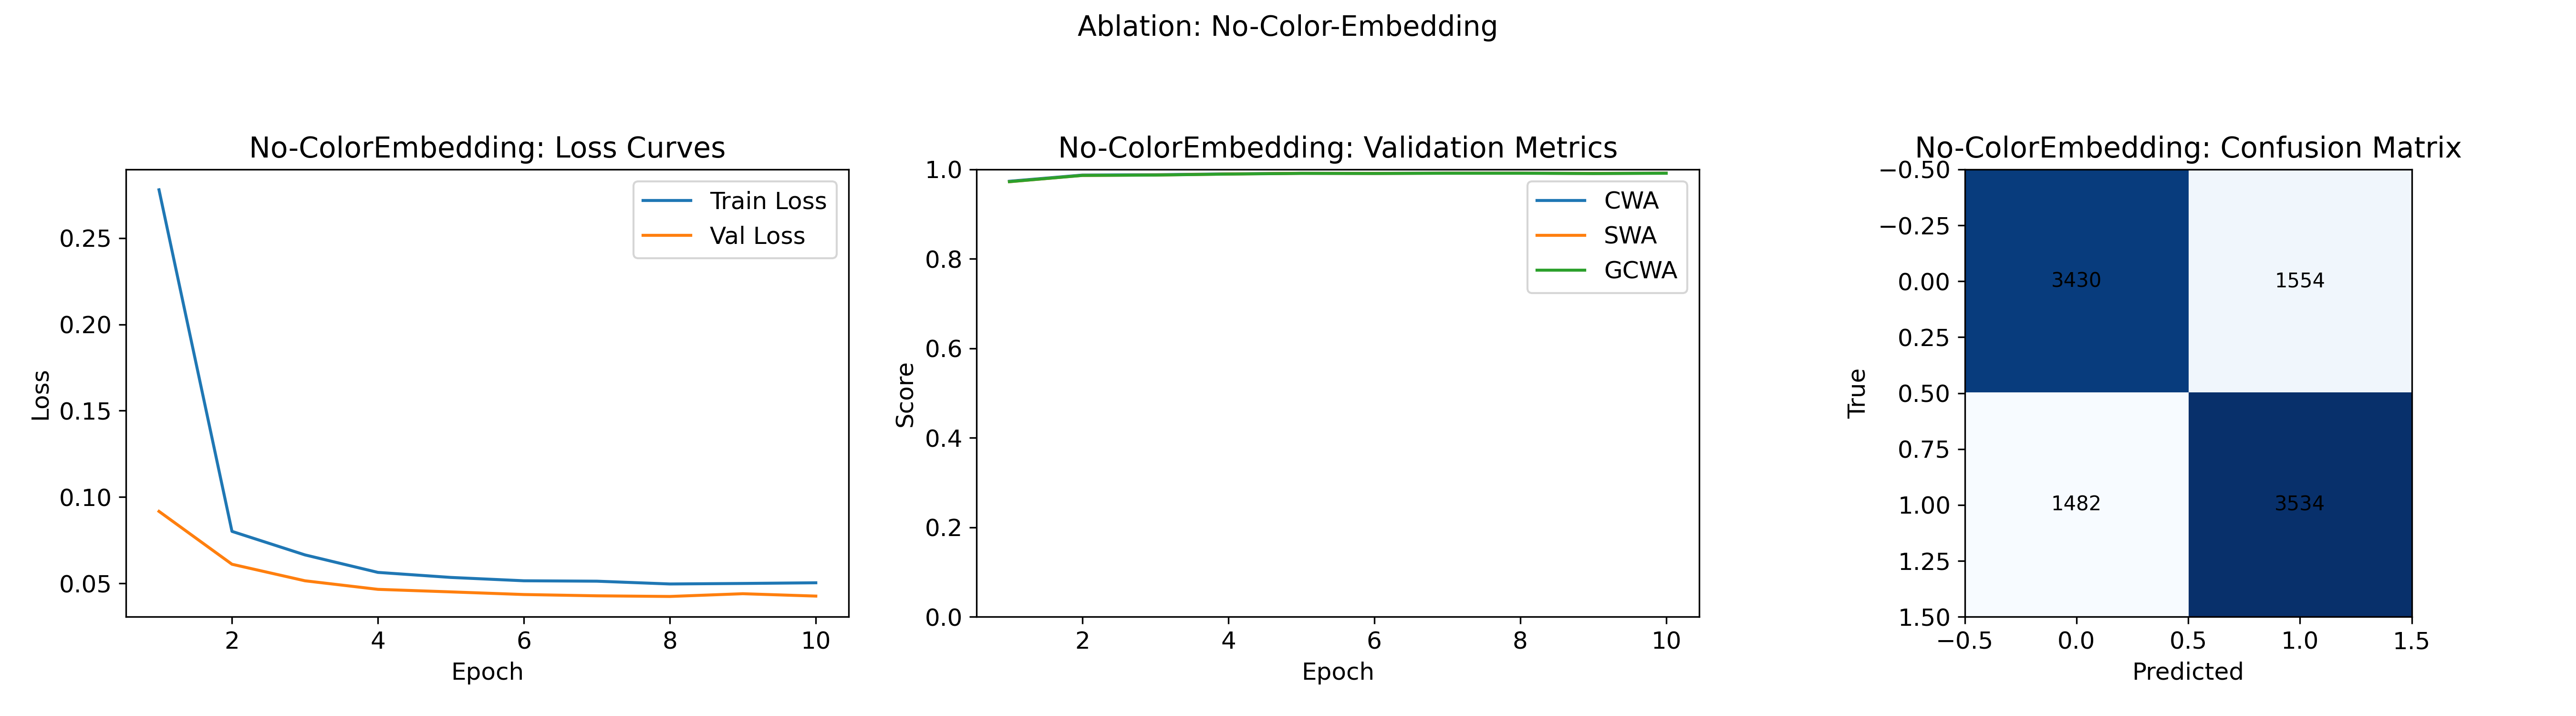
\includegraphics[width=0.24\textwidth]{ablation_no_color_embedding.png}\label{fig:ablations5}}
\subfigure[Random clustering]{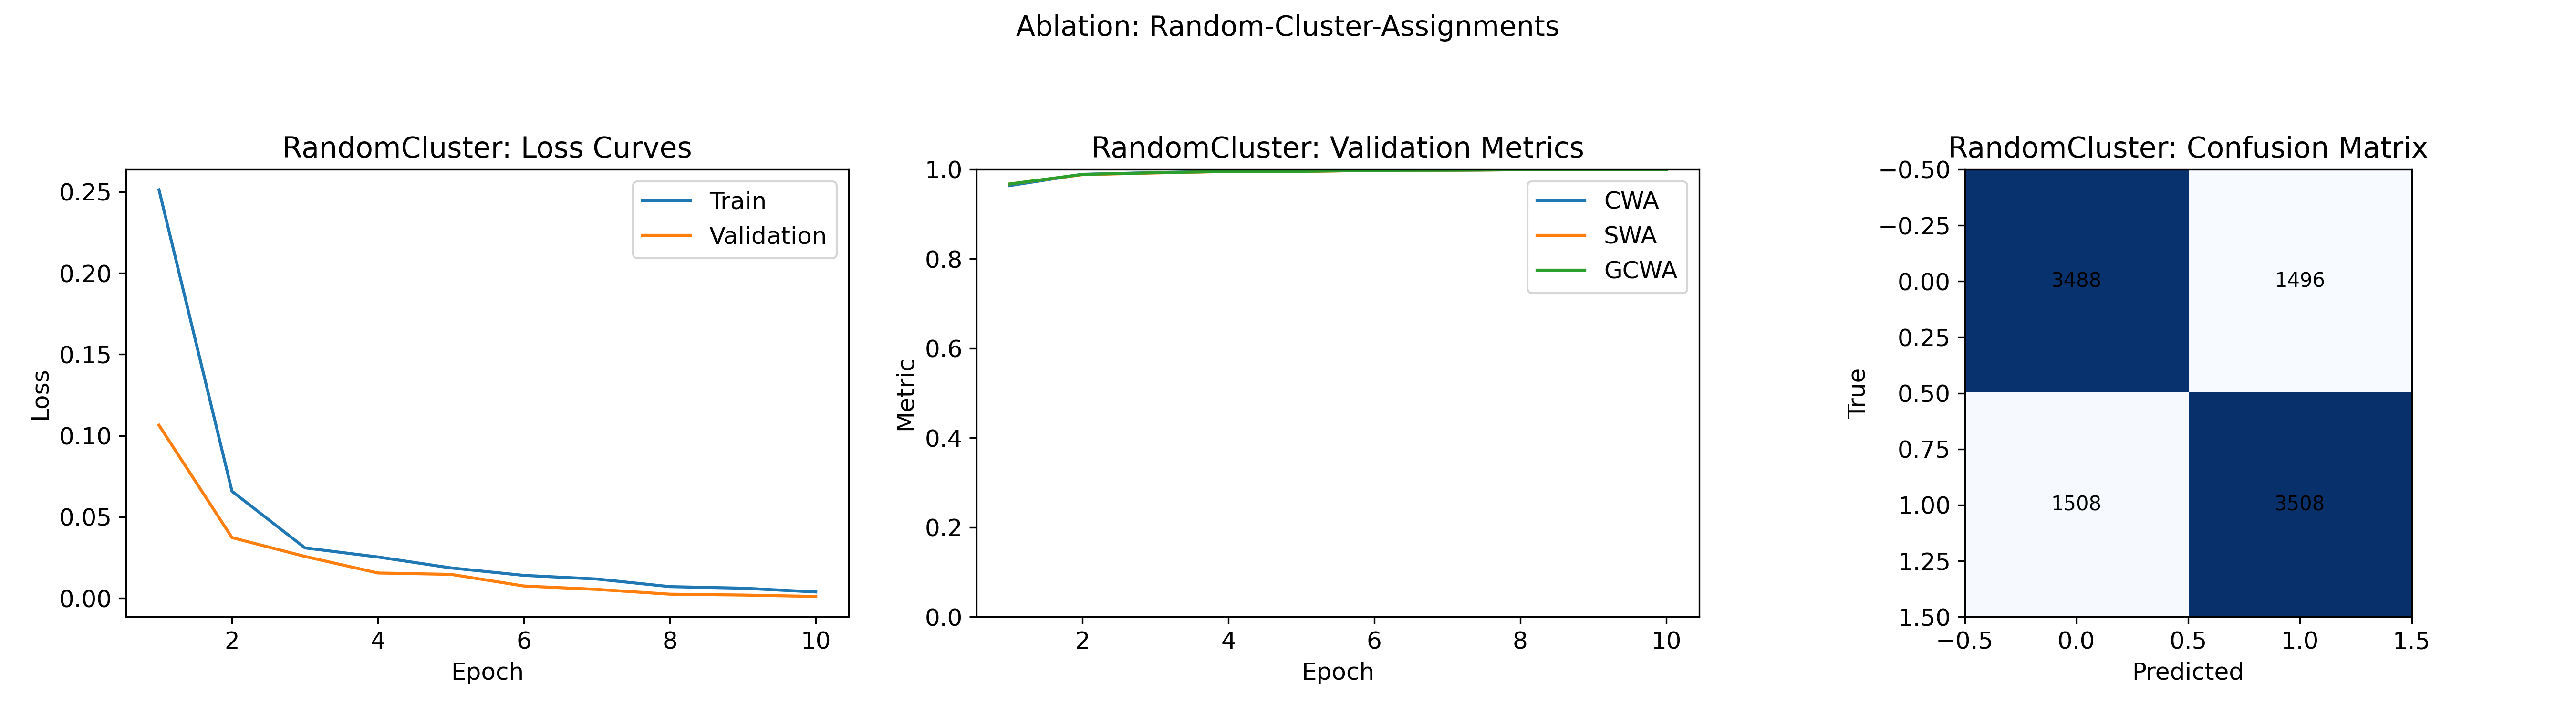
\includegraphics[width=0.24\textwidth]{ablation_random_cluster.png}\label{fig:ablations6}}
\subfigure[Sum-fusion embeddings]{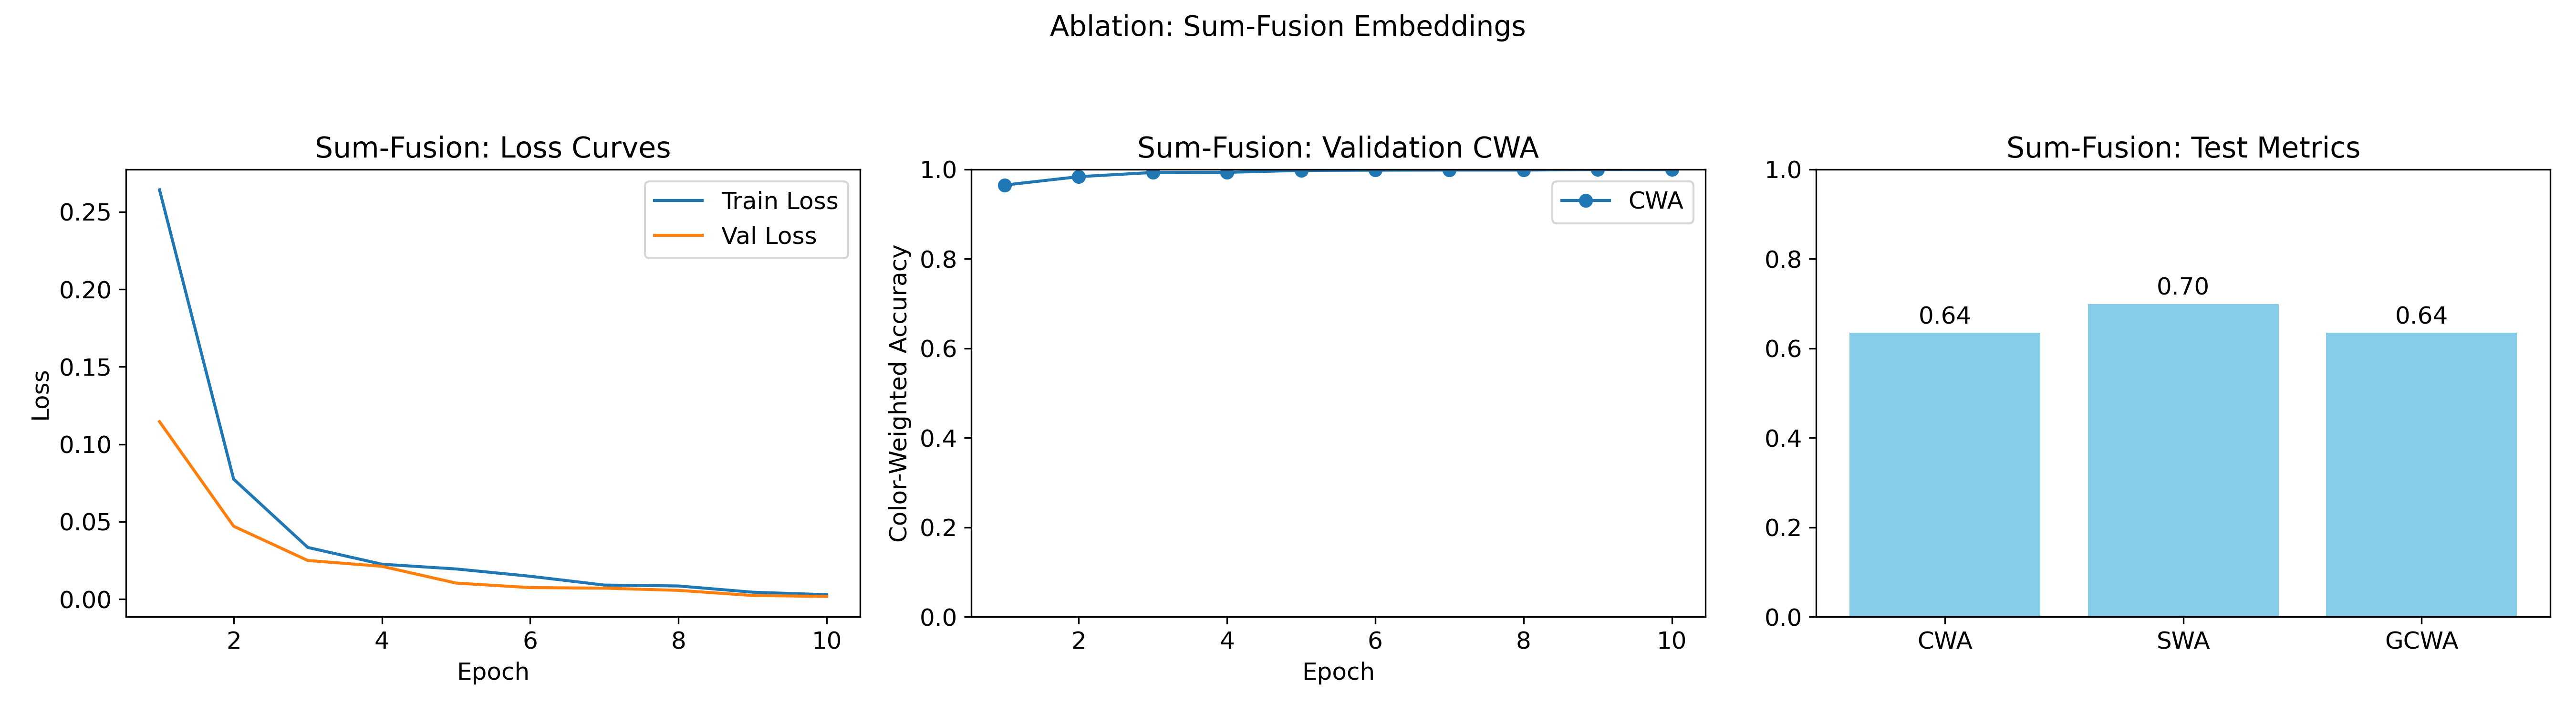
\includegraphics[width=0.24\textwidth]{ablation_sum_fusion_embeddings.png}\label{fig:ablations7}}
\subfigure[Unidirectional LSTM]{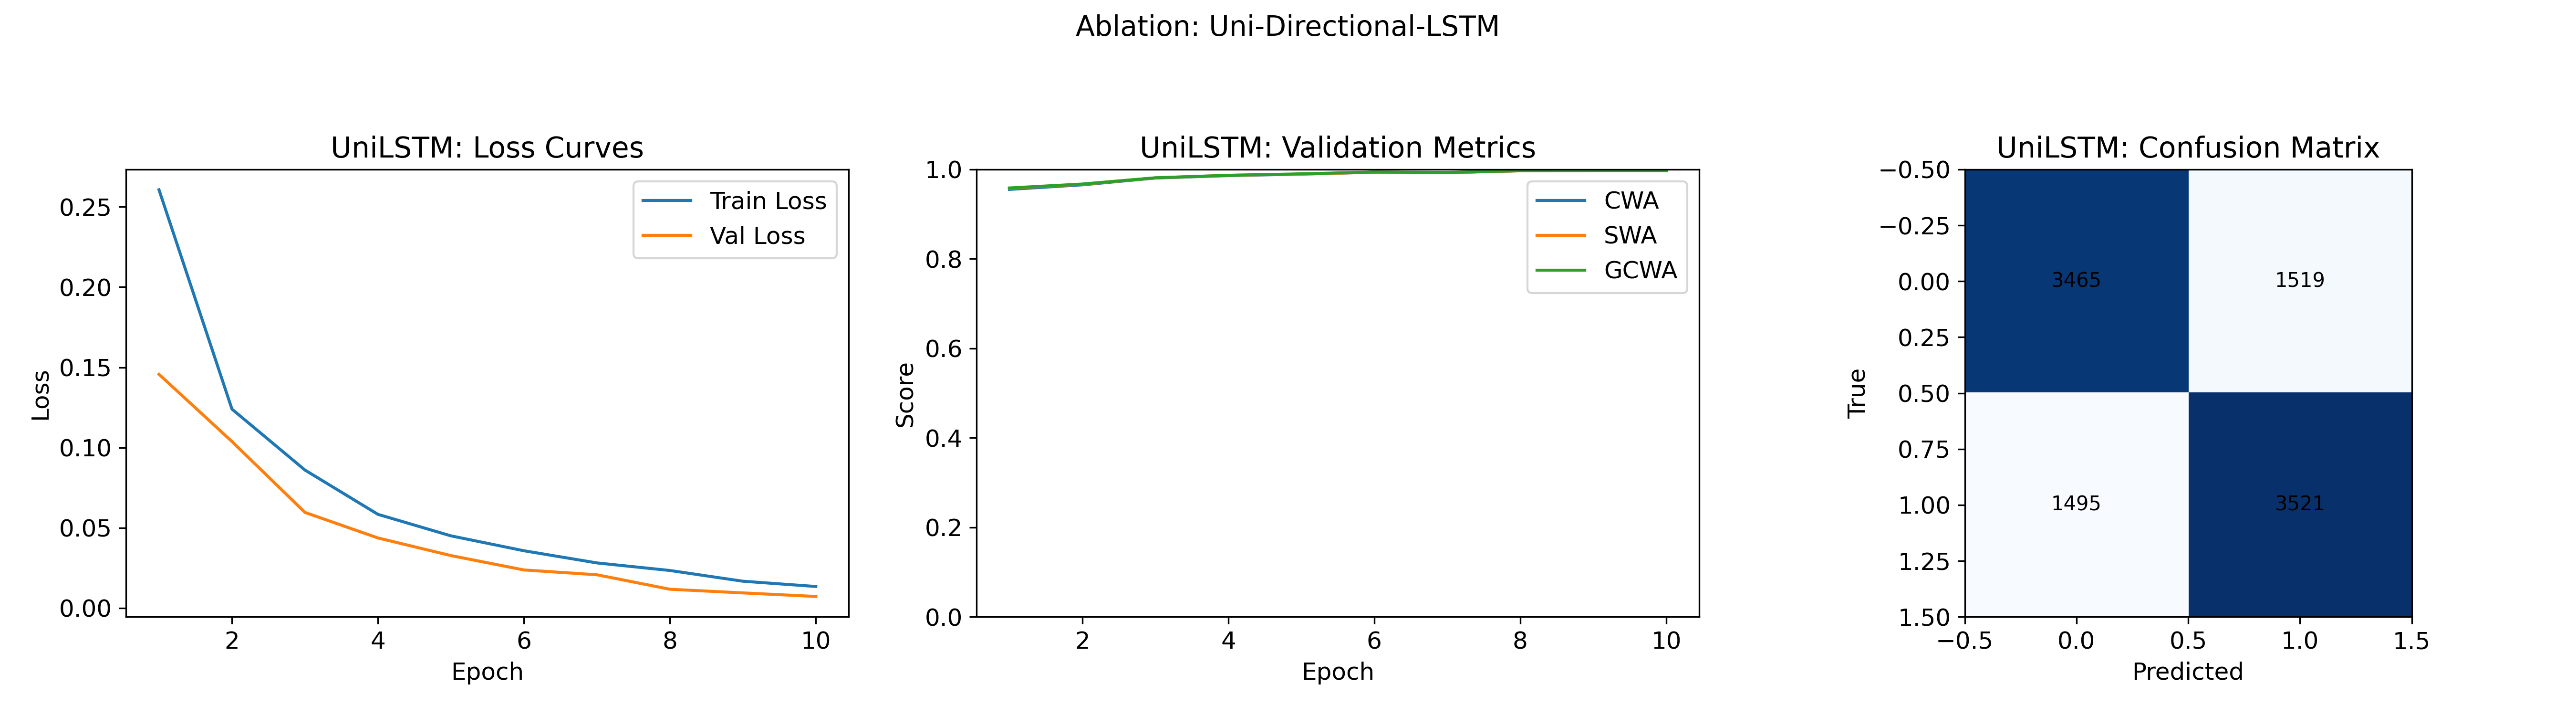
\includegraphics[width=0.24\textwidth]{ablation_uni_lstm.png}\label{fig:ablations8}}
\caption{\textbf{Figure 2: Ablation studies with various configurations.} Each subfigure highlights how a specific design change (e.g., removing color embeddings or applying random clustering) impacts shape and color performance. Removing color embeddings (e) severely diminishes color-based accuracy, while random clustering (f) degrades both shape and color metrics, illustrating the sensitivity of symbolic reasoning to clustering initialization.}
\label{fig:allablations}
\end{figure}